Раздел имеет две части представление языка и его генерация.

\begin{figure}[h]
    \centering
    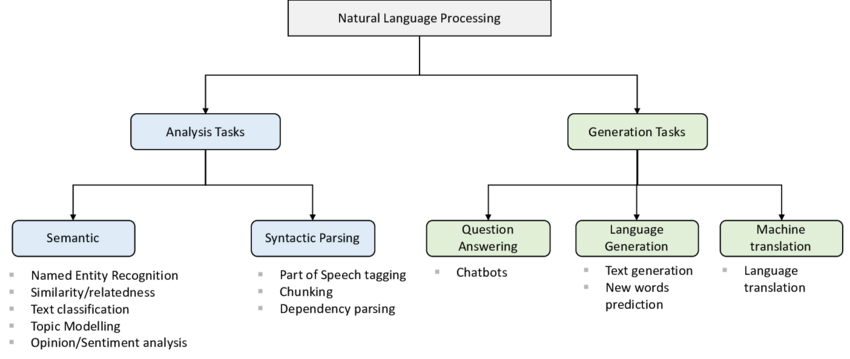
\includegraphics[width=0.5\textwidth]{assets/nlp/taxonomy.png}
    \caption{Таксономия современных подходов обработки естественного языка}
    \label{llm_taxonomy}
\end{figure}

Анализ естественного языка это межпредметная дисциплина.


\subsection{Представление}

\subsection{Лемматизация}

Лемматизация представляет собой процесс нормализации текста, целью которого является приведение слов к их базовой форме или лемме. В контексте обработки естественного языка (Natural Language Processing, NLP), лемматизация является важным этапом предварительной обработки текста, который позволяет уменьшить размер словаря и улучшить качество анализа.

Формально, лемматизация выражается в преобразовании слова \( w \) в его лемму \( \text{lemma}(w) \) с использованием правил и алгоритмов, учитывающих морфологические особенности языка. Лемма представляет собой каноническую, нормализованную форму слова, которая может быть использована для обобщения различных грамматических форм одного и того же слова.

Математически, процесс лемматизации может быть представлен как отображение слова \( w \) в его лемму \( \text{lemma}(w) \):

\[ \text{lemma}(w) = \text{лемма} \]

Например, для слова "бегу", его леммой будет слово "бежать". Лемматизация помогает уменьшить словарь слов и снизить размерность пространства признаков в текстовых данных, что положительно влияет на производительность алгоритмов обработки текста, таких как классификация или кластеризация.

Применение лемматизации часто сопровождается предварительным шагом токенизации, в котором текст разбивается на отдельные слова или токены. Это позволяет применить лемматизацию к каждому слову в тексте независимо от контекста. Лемматизация часто используется в различных областях NLP, включая информационный поиск, анализ тональности, машинный перевод и другие.

\subsection{Векторное представление}


Практически востребованной оказалась дистрибутивная гипотеза \cite{Schutze},
легшая в основу алгоритма \cite{NIPS2013_9aa42b31}.

В генеративном моделировании естественного языка, встает задача представления слов в виде векторов в многомерном пространстве, что позволяет моделировать семантические и синтаксические аспекты текста в компактной форме. Это представление, известное как "векторное вложение" или "embedding", позволяет выразить смысловые и лингвистические свойства слов, используемых в языке.

Формально, векторное вложение \( \mathbf{e}_w \) слова \( w \) представляет собой векторное представление этого слова в многомерном пространстве:

\[ \mathbf{e}_w = (e_{w1}, e_{w2}, ..., e_{wd}) \]

где \( d \) - размерность пространства вложения (число измерений), \( e_{wj} \) - \( j \)-ая компонента вектора вложения \( \mathbf{e}_w \).

Эти векторные представления обычно изучаются и извлекаются из больших корпусов текстов с использованием различных алгоритмов, таких как word2vec, GloVe (Global Vectors for Word Representation), FastText и другие. Они обладают свойством сохранения семантической близости слов в пространстве вложения: слова, которые часто встречаются в похожих контекстах, имеют близкие векторные представления.

Векторные вложения слов играют важную роль в генеративном моделировании естественного языка, так как они позволяют моделям представлять слова в виде непрерывных числовых значений, которые могут быть использованы как входные данные для алгоритмов машинного обучения. Это позволяет моделям эффективно изучать зависимости между словами и генерировать тексты семантически богатые и лингвистически осмысленные.





\subsection{Генерация}

\subsection{N-граммы}

N-граммы представляют собой последовательности из \( n \) элементов в тексте или последовательности символов, где \( n \) обозначает количество элементов в последовательности. Элементы могут быть символами, словами или более крупными фрагментами текста в зависимости от контекста применения. Анализ n-грамм является важным методом в обработке естественного языка (Natural Language Processing, NLP) для изучения частотности последовательностей слов или символов в текстовых данных.

Формально, n-грамма \( \text{ngram}_n \) длины \( n \) в тексте \( T \) определяется как последовательность \( n \) элементов, где каждый элемент \( x_i \) может быть символом, словом или другими единицами текста:

\[ \text{ngram}_n = (x_1, x_2, ..., x_n) \]

Использование n-грамм в анализе текста позволяет оценивать частотность последовательностей слов или символов и изучать лингвистические характеристики текста, такие как структура, стиль и тематика. Кроме того, n-граммы могут использоваться в задачах моделирования языка, предсказания следующего слова в предложении, а также в машинном переводе и других приложениях обработки естественного языка.

\subsection{Авторегрессионая модель}


Авторегрессионные модели в генеративном моделировании естественного языка представляют собой класс статистических моделей, которые моделируют вероятностное распределение последовательности слов или символов в тексте. Эти модели базируются на предположении о зависимости текущего элемента последовательности от предыдущих элементов, что позволяет им учитывать контекст и последовательность в текстовых данных.

Формально, в авторегрессионной модели вероятность появления последовательности \( W = (w_1, w_2, ..., w_T) \) слов или символов определяется как произведение вероятностей каждого слова при условии предыдущих:

\[ P(W) = P(w_1) \cdot P(w_2|w_1) \cdot P(w_3|w_1, w_2) \cdot \ldots \cdot P(w_T|w_1, w_2, ..., w_{T-1}) \]

где \( P(w_t|w_1, w_2, ..., w_{t-1}) \) - вероятность появления слова \( w_t \) при условии всех предыдущих слов \( w_1, w_2, ..., w_{t-1} \).

Авторегрессионные модели могут быть реализованы с использованием различных подходов, включая марковские модели, рекуррентные нейронные сети и модели с авторегрессионными свойствами, такие как GPT (Generative Pre-trained Transformer) и LSTM (Long Short-Term Memory). Они находят применение в широком спектре задач обработки естественного языка, включая генерацию текста, машинный перевод, синтез речи и другие.

Одной из ключевых особенностей авторегрессионных моделей является их способность учитывать контекст и последовательность слов в тексте, что позволяет им генерировать качественные тексты с учетом структуры и семантики. Тем не менее, выбор подходящей модели и обучение ее требуют значительных вычислительных ресурсов и экспертных знаний в области машинного обучения и обработки естественного языка.

\subsection{Attention}

Механизм внимания (attention) в генеративном моделировании естественного языка является ключевым компонентом в нейронных сетях, позволяющим модели фокусироваться на определенных частях входных данных при выполнении задач обработки текста. Этот механизм позволяет модели адаптироваться к различным контекстам и динамически выделять важные элементы во входных последовательностях.

Формально, предположим, что у нас есть входные данные \( X = (x_1, x_2, ..., x_T) \) и контекст \( C \), а также текущее состояние скрытого слоя модели \( h_t \). Механизм внимания вычисляет вектор внимания \( \alpha \), который определяет важность каждого элемента входной последовательности на текущем временном шаге:

\[ \alpha_t = \text{softmax}(f(h_t, X)) \]

где \( f \) - функция, которая вычисляет важность каждого элемента входной последовательности, а \( \text{softmax} \) применяется для получения нормированных весов внимания.

С использованием вектора внимания \( \alpha \), взвешенная сумма контекста \( C \) вычисляется как:

\[ context_t = \sum_{i=1}^{T} \alpha_{ti} x_i \]

Полученный контекст используется в дальнейших вычислениях модели для выполнения задач, таких как генерация текста или классификация.

Механизм внимания позволяет модели сосредоточиться на наиболее значимых частях входных данных в каждый момент времени, что делает его особенно полезным для задач, требующих адаптивности и контекстного понимания, таких как машинный перевод, генерация текста и вопросно-ответные системы. Этот механизм стал ключевым инструментом в области генеративного моделирования естественного языка, позволяя моделям эффективно работать с различными типами данных и контекстами.

